%APPENDIX
\begin{appendices}

\chapter{Results for composite rational functions}\label{compratappendix}

This appendix will contain results relating to composite rational functions. As such, we will briefly discuss some definitions and examples---similar to those seen in the preliminary discussion in a polynomial setting---involving rational functions.

\section{Composite rational functions and degrees of freedom} 

\begin{defn}
The \textit{degrees of freedom} of a rational function $r_{m,n} \in \Arr_{m,n}$ is the number of parameters required to completely determine $r_{m,n}$. We say that $r_{m,n}$ is a \textit{plain rational function} if $r_{m,n}$ has $m+n+1$ degrees of freedom, i.e.
\[r_{m,n}(x) = \dfrac{\sum_{k=0}^m \alpha_k x^k}{1+\sum_{k=1}^n \beta_k x^k},\]
for some independent scalars $\alpha_k, \beta_k \in \R$.
\end{defn}

\begin{defn}\label{compratdef}
A bivariate rational function $r(x,y)$ is said to be of type $(m,n)$ if $r(x,x) \in \Arr_{m,n}$. A rational function $r(x)$ is said to be \textit{$(k,m,n)$-composite} if
\begin{align}
    r(x) = r_k(x,r_{k-1}(x,r_{k-2}(\cdots(x,r_1(x,1))))) \label{rat}
\end{align}
for bivariate rational functions $r_i(x,y)$, $i=1,\dots,k$, each of type $(m,n)$. We say that a $(k,m,n)$-composite rational function is $pure$ if the $r_i(x,y)$ in \eqref{rat} are univariate, i.e. $r(x) = r_k(r_{k-1}(\cdots(r_1(x))))$.
\end{defn}

\begin{ex}
A rational function of the form \eqref{rat} has at most $k(m+n+1)$ degrees of freedom. In particular, a pure composite rational function of the form $r(x)=r_k(\cdots r_2(r_1(x)))$ with each $r_i$ of type $(n,n)$ is of type $(n^k,n^k)$, but has $d\approx 2kn$ degrees of freedom.
\end{ex}

Examples of composite rational functions we have encountered throughout this dissertation include the Newton iterates for the sign and square root functions, and more subtly the Zolotarev functions.

\section{Composite rational approximation to \texorpdfstring{$\sqrt{x}$}{sqrt(x)}}

The motivation for the novel part of this dissertation, namely the construction of a composite polynomial approximation to $\sqrt{x}$, stemmed from the work of Gawlik and Nakatsukasa \cite{Yuji} concerning the composite rational approximation of $x^{1/p}$ on $[\alpha^p,1]$ for some $\alpha \in (0,1)$. In this appendix, we present their results for $p=2$, and simplify proofs where possible. 

\begin{thm}\label{squareroot}
There exists $N \in \N$ such that for every integer $n \geq N$, there is a rational function $r \in \Arr_{n,n-1}([0,1])$, which is a composition of $\lfloor\log_2 n\rfloor+1$ type-$(2,1)$ rational functions, and a constant $C>0$ such that
\[\max_{x\in[0,1]}|r(x)-\sqrt{x}| \leq \exp(-C\sqrt{n}).\]
\end{thm}

Theorem \ref{squareroot} implies that the convergence of $r$ to $\sqrt{x}$ is \textit{doubly exponential} with respect to $d$, the number of degrees of freedom, as $n\to\infty$. That is, for constants $C_1,C_2>0$, the error is $O(\exp(-C_1\exp(C_2 d)))$, where $d\approx 4\log_2 n$. To prove Theorem \ref{squareroot}, we consider
\begin{align}
    f_{k+1}(x)=\dfrac{1}{2}\left(\sqrt{\alpha_k}f_k(x)+\dfrac{x}{\sqrt{\alpha_k} f_k(x)}\right), \qquad f_0(x)=1, \label{theiter}
\end{align}
where throughout this appendix we define the sequence $(\alpha_k)$ by 
\[\alpha_{k+1}=\dfrac{2\sqrt{\alpha_k}}{1+\alpha_k},\qquad \alpha_0=\alpha.\]
Note that $f_k$ is $(k,2,1)$-composite with 
\[r_j(x,y)=\dfrac{1}{2}\left(\dfrac{\alpha_{j-1}y^2+x}{\sqrt{\alpha_{j-1}}y}\right), \qquad j=1,\dots,k.\]
A simple induction shows that $f_k \in \Arr_{2^{k-1},2^{k-1}-1}$ for each $k\geq 1$. In what follows, we will approximate the square root function with the scaled functions
\[\tilde{f}_k(x)=\dfrac{2\alpha_k}{1+\alpha_k}f_k(x),\]
which in particular have the same number of degrees of freedom of the $f_k$. We will prove the following result, which will enable us to show that the $\tilde{f}_k$ converge to $\sqrt{x}$ at a doubly exponential rate with respect to the degrees of freedom.

\begin{thm}\label{fsquig}
For any $k \in \N$, $\alpha \in (0,1)$, there holds
\[\max_{x\in[0,1]}|\tilde{f}_k(x)-\sqrt{x}| \leq \max\left\{2\alpha,\dfrac{1-\alpha_k}{1+\alpha_k}\right\}.\]
\end{thm}

\subsection{Bounding the error on \texorpdfstring{$[0,\alpha^2]$}{[0,a2]}}

To prove Theorem \ref{fsquig}, we consider the error over $[0,\alpha^2]$ and $[\alpha^2,1]$ separately. In this section, we consider the first interval and prove the following error bound.

\begin{thm}\label{0bound}
For any $k \in \N$, $\alpha \in (0,1)$, there holds
\[\max_{x\in [0,\alpha^2]}|\tilde{f}_k(x)-\sqrt{x}|\leq 2\alpha.\]
\end{thm}

To prove this, we need a few lemmas. We first define the functions
\[s_\alpha(x):= \dfrac{2x\sqrt{\alpha}}{\alpha+x^2}, \qquad H(\alpha):= s_\alpha(\alpha) = \dfrac{2\sqrt{\alpha}}{1+\alpha}, \qquad g_k(x):= \dfrac{x}{f_k(x^2)},\]
and note that
\begin{align}
    H(\alpha_k)=\alpha_{k+1}, \qquad g_{k+1}(x) = s_{\alpha_k}(g_k(x)). \label{geekay}
\end{align}

\begin{lemma}\label{A3}
For any $\alpha \in (0,1)$, $x \in [0,\alpha]$, we have
\[0 \leq x s'_\alpha(x) \leq s_\alpha(x) \leq H(\alpha).\]
\end{lemma}

\begin{proof}
Since $s_\alpha$ is nondecreasing on $[0,\alpha]$, we have 
\[0\leq xs'_\alpha(x), \qquad s_\alpha(x) \leq H(\alpha).\]
Furthermore, we can compute
\[xs'_\alpha(x) = \left(\dfrac{\alpha-x^2}{\alpha+x^2}\right)\left(\dfrac{2x\sqrt{\alpha}}{\alpha+x^2}\right)\leq s_\alpha(x)\]
since $0\leq \frac{\alpha-x^2}{\alpha+x^2}\leq 1$ for all $x \in [0,\alpha] \subset [0,\sqrt{\alpha}]$. 
\end{proof}

\begin{lemma} \label{ggkk}
For any $k \in \N$, $\alpha \in (0,1)$, $x \in [0,\alpha]$, we have
\begin{align}
    0 \leq x g'_k(x) \leq g_k(x) \leq \alpha_k.\label{lem2}
\end{align}
\end{lemma}

\begin{proof}
By induction. The case $k=0$ is clear since $g_0(x)=x$ and $\alpha_0=\alpha$. Now assume that \eqref{lem2} holds for $k=n$. By \eqref{geekay}, we have
\[xg'_{n+1}(x)=xs'_{\alpha_n}(g_n(x))g'_n(x).\]
As $0\leq g_n(x)\leq \alpha_n$ by the induction hypothesis, Lemma \ref{A3} with $\alpha=\alpha_n$ implies that $xg'_{n+1}(x)\geq 0$ for $x \in [0,\alpha]$. The lemma further shows that
\[xg'_{n+1}(x) \leq s'_{\alpha_n}(g_n(x))g_n(x) \leq s_{\alpha_n}(g_n(x)) = g_{n+1}(x).\]
Finally, as noted in Lemma \ref{A3},
\[g_{n+1}(x) = s_{\alpha_n}(g_n(x)) \leq H(\alpha_n) = \alpha_{n+1},\]
which completes the inductive step.
\end{proof}

\begin{lemma}\label{finallem}
For any $k \in \N$, $\alpha \in (0,1)$, $x \in [0,\alpha^2]$, we have
\[0 < \tilde{f}_k(x) \leq \alpha(1+\ep_k), \qquad \text{where}\qquad  \ep_k=\dfrac{1-\alpha_k}{1+\alpha_k}.\]
\end{lemma}

%Induction: f_k > 0 easy, f_k non-decreasing ok: clear for k=0, assume y>x and show f_k+1(y) >= f_k+1(x) 

\begin{proof}
A simple induction shows that $f_k(x)>0$ is non-decreasing on $[0,\alpha^2]$ for every $k$. Writing $f_k(x^2)=x/g_k(x)$, we differentiate to obtain
\[2xf'_k(x^2) = \dfrac{g_k(x)-xg'_k(x)}{g_k(x)^2} \geq 0\]
by Lemma \ref{ggkk}. Hence $f'_k(x^2)\geq 0$ for $x \in [0,\alpha^2]$. Setting \eqref{theiter} at $x=0$ gives
\[f_{k+1}(0)=\dfrac{\sqrt{\alpha_k}}{2}f_k(0), \qquad f_0(0)=1,\]
so $0<f_k(0)\leq f_k(x)$ on $[0,\alpha^2]$ for every $k$, and so $0<\tilde{f}_k(x)\leq \tilde{f}_k(\alpha^2)$ as $\tilde{f}_k$ is a positive multiple of $f_k$. The upper bound on $\tilde{f}_k$ is obtained by \cite[Theorem 3.1]{Gawlik}, which provides the relative error bound
\[\max_{x\in[\alpha^2,1]}\dfrac{\tilde{f}_k(x)-\sqrt{x}}{\sqrt{x}}=\dfrac{1-\alpha_k}{1+\alpha_k}=\ep_k.\]
Taking $x=\alpha^2$ gives $\tilde{f}_k(\alpha^2) \leq \alpha(1+\ep_k)$, as required.
\end{proof}

We are now in a position to prove Theorem \ref{0bound}, from which we can quickly deduce the result of Theorem \ref{fsquig}.

\begin{proof}[Proof of Theorem \ref{0bound}]
By Lemma \ref{finallem}, we have for $x\in [0,\alpha^2]$
\begin{align*}
    |\tilde{f}_k(x)-\sqrt{x}| &\leq \max\{|\tilde{f}_k(x)|,|\sqrt{x}|\}\\
    &\leq \max\{\alpha(1+\ep_k),\alpha\}\\
    &=\alpha(1+\ep_k)\\
    &\leq 2\alpha,
\end{align*}
since $\ep_k \in (0,1)$. Thus $\max_{x\in[0,\alpha^2]}|\tilde{f}_k(x)-\sqrt{x}|\leq 2\alpha$, as required.
\end{proof}

\begin{proof}[Proof of Theorem \ref{fsquig}]
If we combine the result of \cite[Theorem 3.1]{Gawlik} with Theorem \ref{0bound}, we obtain
\begin{align*}
    \max_{x\in[0,1]}|\tilde{f}_k(x)-\sqrt{x}| &=\max\left\{2\alpha,\max_{x\in[\alpha^2,1]}|\tilde{f}_k(x)-\sqrt{x}|\right\}\\
    & \leq \max \left\{2\alpha,\max_{x\in[\alpha^2,1]}\left|\dfrac{\tilde{f}_k(x)-\sqrt{x}}{\sqrt{x}}\right|\right\}\\
    & = \max\left\{2\alpha,\dfrac{1-\alpha_k}{1+\alpha_k}\right\},
\end{align*}
as required.
\end{proof}

\subsection{Proof of Theorem \texorpdfstring{\ref{squareroot}}{(4.1)}}

Theorem \ref{fsquig} is used in \cite{Yuji} as a basis for the analysis of the convergence of $\tilde{f}_k$ to $\sqrt{x}$ on $[0,1]$, and ultimately proving Theorem \ref{squareroot}. Nakatsukasa and Gawlik take a constructive approach to determining, for arbitrary $\ep>0$, values of $\alpha$, $k$ such that $\max_{x\in[0,1]}|\tilde{f}_k(x)-\sqrt{x}|< \ep$. By Theorem \ref{fsquig}, we must have $\alpha \leq \ep/2$ and $k$ large enough such that $\ep_k \leq \ep$. We determine $k$ in three steps:

\begin{enumerate}
    \item[(1)] Find $k_1$ such that $\alpha_{k_1} \geq 1/e$;
    \item[(2)] Select $\alpha^* \in (1/e,1)$ and find $k_2$ such that $\alpha_{k_1+k_2} \geq \alpha^*$;
    \item[(3)] Find $k_3$ such that $\ep_{k_1+k_2+k_3}\leq \ep$. 
\end{enumerate}

%\begin{figure}[t!]
%\centering
%   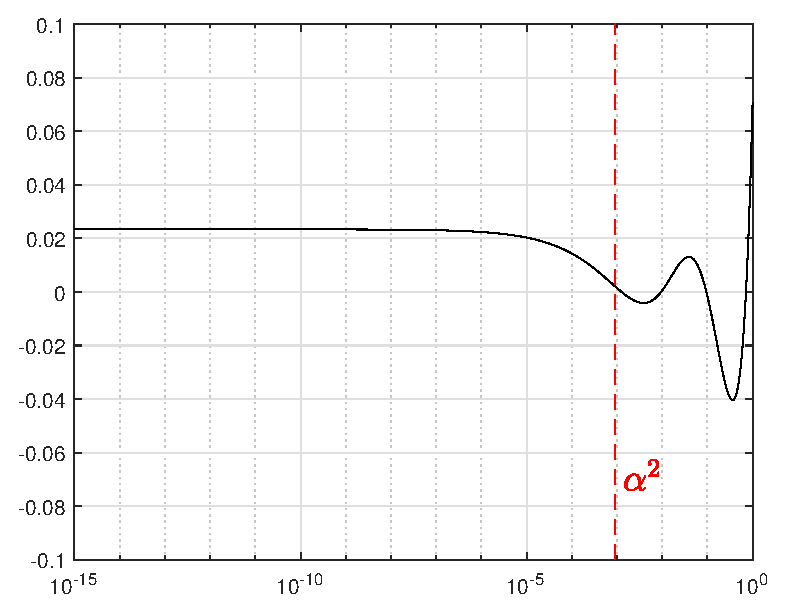
\includegraphics[scale=0.8]{Comp_sqrt_approx_withline.eps}
%   \caption{Error curve $E(x)=\tilde{f}_2(x)-\sqrt{x}$ for $\alpha=0.03$. Note that the error on $[0,\alpha^2]$ is bounded by that on $[\alpha^2,1]$, which is $\ep=2\alpha$.}
%   \label{fig:alpha}
%\end{figure}

Then $k\geq k_1+k_2+k_3$. The choice of $\alpha^*$ in step 2 is given by $\delta^*$ in Lemma \ref{hh}.

\bigskip{}

\textbf{Step 1.} To determine $k_1$ such that $\alpha_{k_1}\geq 1/e$, we first note that $\alpha_{k+1}> \sqrt{\alpha_k}$. To see this, we can argue by contradiction (a much simpler proof than that of Nakatsukasa and Gawlik). If $\alpha_{k+1} \leq \sqrt{\alpha_k}$, then
\begin{align*}
    \dfrac{2\sqrt{\alpha_k}}{1+\alpha_k}\leq \sqrt{\alpha_k} \qquad \Longrightarrow\qquad 2\sqrt{\alpha_k} &\leq \sqrt{\alpha_k} + \alpha_k\sqrt{\alpha_k} < 2\sqrt{\alpha_k},
\end{align*}
since $\alpha_k \in(0,1)$, a contradiction. Hence $\alpha_{k+1}>\sqrt{\alpha_k}$ for all $k$, so
\[\alpha_k \geq \alpha_0^{(1/2)^k}=\alpha^{(1/2)^k}.\]
Thus we will have $\alpha_{k_1}\geq 1/e$ if $\alpha^{(1/2)^{k_1}}\geq 1/e$, namely
\[k_1\geq \dfrac{\log\log \frac{1}{\alpha}}{\log 2}.\]
Since $\alpha\leq \ep/2$ is assumed, we can write a lower bound in terms of $\ep$, i.e.
\[k_1 \geq \dfrac{\log\log \frac{2}{\ep}}{\log 2}.\]

\textbf{Step 2.} We pick $\alpha^*$ such that the result of Lemma \ref{hh} holds. Note that $k_2$ is independent of $\ep$ and $\alpha$, hence constant.

\bigskip{}

\textbf{Step 3.} To determine $k_3$ such that $\ep_{k_1+k_2+k_3} \leq \ep$, we note that
\[\ep_{k+1}=\dfrac{1-H(\alpha_k)}{1+H(\alpha_k)}\leq \left(\dfrac{1-\alpha^*}{1+\alpha^*}\right)^2\]
for $k\geq k_1+k_2$ by Lemma \ref{hh}. In particular,
\[\ep_{k_1+k_2+k}\leq \ep_{k_1+k_2}^{2^k}\leq \left(\dfrac{1-\alpha^*}{1+\alpha^*}\right)^{2^k},\]
so $\ep_{k_1+k_2+k_3}\leq \ep$ if $k_3$ is chosen such that
\[k_3 \geq \dfrac{\log\log\frac{1}{\ep}-\log\log\frac{1+\alpha^*}{1-\alpha^*}}{\log 2}.\]

Combining the steps, we find that $\max_{x\in[0,1]}|\tilde{f}_k(x)-\sqrt{x}|< \ep$ when
\[k \geq \dfrac{\log\log\frac{2}{\ep}}{\log 2} + k_2 + \dfrac{\log\log\frac{1}{\ep}-\log\log\frac{1+\alpha^*}{1-\alpha^*}}{\log 2}.\]

We now prove Theorem \ref{squareroot}, simplifying the version provided in \cite{Yuji}.

\begin{proof}[Proof of Theorem \ref{squareroot}]
As previously mentioned, $\tilde{f}_k$ will be a type $(2^{k-1},2^{k-1}-1)$ rational function. Define 
\[\tilde{k}_2=\left\lfloor k_2-\frac{\log\log \frac{1+\alpha^*}{1-\alpha^*}}{\log 2}\right\rfloor,\]
so that the degree $n=2^{k-1}$ of the iteration $\tilde{f}_k$ which approximates $\sqrt{x}$ with accuracy $\ep$ can be given by
\begin{align*}
    \log n= (k-1)\log 2 &= \left(\dfrac{\log\log\frac{2}{\ep}+\log\log\frac{1}{\ep}}{\log 2}+\tilde{k}_2\right)\log 2\\
    & \leq \left(\dfrac{2\log\log\frac{2}{\ep}}{\log 2}+\tilde{k}_2\right)\log 2,
\end{align*}
after absorbing the constant $-1$ into $\tilde{k}_2$. Hence
\[\log\log \dfrac{2}{\ep}\geq \dfrac{\log n - \tilde{k}_2 \log 2}{2},\]
which further simplifies to give
\[\ep \leq 2\exp(-C\sqrt{n}),\]
where $C = 2^{-\tilde{k}_2/2}$. This proves the theorem if the exact degree $n$ is a sufficiently large power of $2$; if $n \not\in \{2^k : k\in \N\}$, then we note that $\left\lfloor \log_2 n\right\rfloor +1$ iterations gives a rational function of type $(2^{\left\lfloor \log_2 n\right\rfloor},2^{\left\lfloor \log_2 n\right\rfloor}-1)$, and for $n \geq N$, the error is bounded by
\begin{align*}
    2\exp(-C(2^{\left\lfloor \log_2 n\right\rfloor})^{1/2}) &\leq 2\exp(-2^{-1/2}Cn^{1/2})\\
    &\leq \exp(-(2^{-1/2}C-N^{-1/2}\log 2)n^{1/2}).
\end{align*}
Taking $N$ so that $2^{-1/2}C-N^{-1/2}\log 2>0$ proves the theorem.
\end{proof}

\end{appendices}